%%%%%%%%%%%%%%%%%%%%%%%%%%%%%%%%%%%%%%%%%
%
% (c) 2022 by Jennifer Laaser
%
% This work is licensed under the Creative Commons Attribution-NonCommercial-ShareAlike 4.0 International License. To view a copy of this license, visit http://creativecommons.org/licenses/by-nc-sa/4.0/ or send a letter to Creative Commons, PO Box 1866, Mountain View, CA 94042, USA.
%
% The current source for these materials is accessible on Github: https://github.com/jlaaser/pogil-polymers
%
%%%%%%%%%%%%%%%%%%%%%%%%%%%%%%%%%%%%%%%%%

\renewcommand{\figpath}{content/polymphys/thermal-transitions/Tg/figs}
\renewcommand{\labelbase}{Tg}

\begin{activity}{The Glass Transition}

\begin{instructornotes}
	This activity introduces students to concepts related to glass transitions of polymer materials.
	
	After completing this activity, students will be able to:
	\begin{enumerate}
		\item ...
	\end{enumerate}
	
	\subsection*{Activity summary:}
	\begin{itemize}
		\item \textbf{Activity type:} Learning Cycle
		\item \textbf{Content goals:} Glass Transitions of Polymer Materials
		\item \textbf{Process goals:} %https://pogil.org/uploads/attachments/cj54b5yts006cklx4hh758htf-process-skills-official-pogil-list-2015-original.pdf
			\begin{enumerate}
				\item Linking concepts to derive a key result
				\item Communication (written and oral) of reasoning
			\end{enumerate}
		\item \textbf{Duration:} TBD
		\item \textbf{Instructor preparation required:} none beyond knowledge of relevant content
		\item \textbf{Related textbook chapters:}
			\begin{itemize}
				\item \emph{Polymer Chemistry} (Hiemenz \& Lodge): section XYZ
			\end{itemize}
		\item \textbf{Instructor notes:}
			\begin{itemize}
				\item \dots
			\end{itemize}
	\end{itemize}
	
\end{instructornotes}


\begin{model}[Free Volume]
	\label{\labelbase:mdl:freevolume}
	
	The following cartoon depicts the changes that happen at the molecular level as a polymer is cooled from high temperature to low temperature:
	
	\centerline{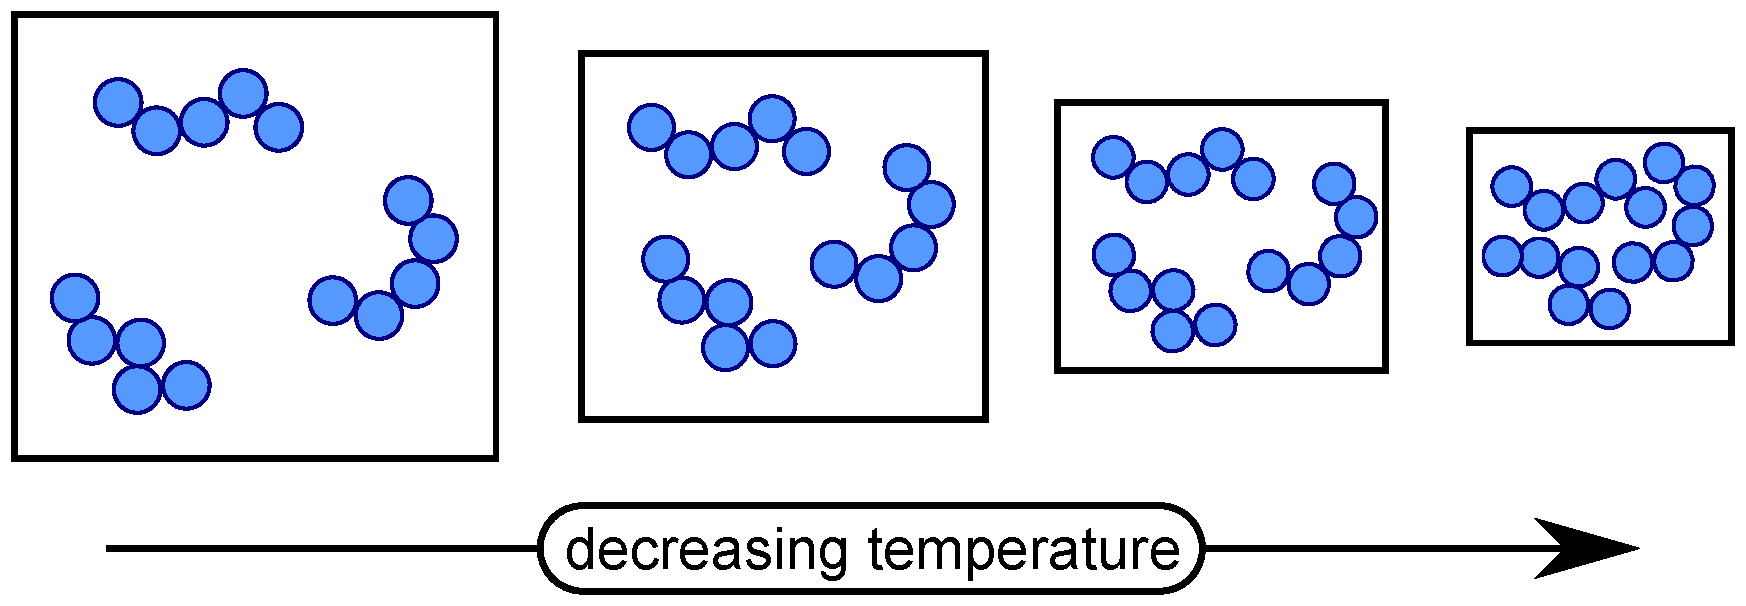
\includegraphics[width=0.7\textwidth]{\figpath/Model1_FreeVolume}}
	
	In this image, the shaded circles represent the \textit{occupied volume} of the polymers, which reflects their van der Waals radii plus the space required for chemical bonds to vibrate.  The white area represents the \emph{free volume} of the material, which is the space available for the molecules to rotate and translate.
	
\end{model}


\begin{ctqs}

	\question Briefly indicate how each of the following changes as the temperature of the sample is lowered:
	
		\begin{enumerate}
		
			\item the occupied volume:
			
				\begin{solution}[0.25in]
				\end{solution}
			
			\item the free volume:
			
				\begin{solution}[0.25in]
				\end{solution}
			
			\item the overall density of the material:
			
				\begin{solution}[0.25in]
				\end{solution}
			
		\end{enumerate}
		
	\question On the following axes, sketch lines depicting how the total volume, $V$, and the occupied volume, $V_{occ}$, change with temperature.  Then, \emph{shade in} the are on the plot that corresponds to the free volume. \label{\labelbase:ctq:VTplot1}
	
		\vspace{0.25in}
		\centerline{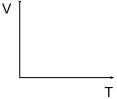
\includegraphics[width=0.35\textwidth]{\figpath/Model1_VTaxes}}
		
	\question As the free volume decreases, it takes more and more time for the polymer chains to rearrange.  How do you expect this to affect... \label{\labelbase:ctq:viscosityconcept}
	
		\begin{enumerate}
			\item ... the relaxation time of the material?
			
				\begin{solution}[0.5in]
				\end{solution}
			
			\item ... the viscosity of the material?
			
				\begin{solution}[0.5in]
				\end{solution}
				
		\end{enumerate}
	
\end{ctqs}

\begin{infobox}

	The viscosity of polymer melts can be described by
	\begin{equation*}
		\eta = A' e^{\frac{B' V_{occ}}{V_f}}
	\end{equation*}
	where $A'$ and $B'$ are constants.  With some rearrangement, and the assumption that the fraction of the material that is free volume increases linearly with temperature, this expression can be rewritten
	\begin{equation*}
		\eta = A e^{\frac{B}{T-T_0}}
	\end{equation*}
	where $T_0$ is the \emph{Vogel temperature}.  This expression is known as the \emph{Vogel-Fulcher-Tamman} (or VFT) \emph{equation}.
	
	In many practical applications, it is more useful to instead express how the viscosity changes relative to a reference temperature.  After some math, it is possible to show that
	\begin{equation*}
		\ln\left(\frac{\eta}{\eta_r}\right) = -\frac{C_1(T-T_r)}{C_2 + (T-T_r)}
	\end{equation*}
	where $\eta_r$ is the viscosity at reference temperature $T_r$ and $C_1$ and $C_2$ are experimentally-determined parameters.  This equation is called the \emph{Williams-Landel-Ferry \emph{(or WLF)} equation.}
			
\end{infobox}

\begin{ctqs}
		
	\question Are these expressions consistent with the trend you predicted in CTQ \ref{\labelbase:ctq:viscosityconcept}?  Briefly explain your group's reasoning.
			
				\begin{solution}[1in]
				\end{solution}
	
	\clearpage
	\question At some temperature, the relaxation time of the material will become so slow that the polymers are effectively unable to keep rearranging to find higher-density/lower free-volume configurations.  After this point, further decreases in the temperature will not significantly change the free volume of the polymer. \label{\labelbase:ctq:traptemp}
	
		Based on this information, propose a revised version of your plot from CTQ \label{\labelbase:ctq:VTplot1} that more accurately depicts changes in the free volume and total volume of a real polymer material.  Make sure the transition temperature is clearly labeled.
	
		\vspace{0.25in}
		\centerline{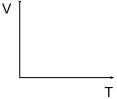
\includegraphics[width=0.35\textwidth]{\figpath/Model1_VTaxes}}
		
	\question Which type of materials properties (liquid-like or solid-like) do you expect to observe in each of the following limits?  Briefly indicate your group's reasoning. \label{\labelbase:ctq:properties}
	
		\begin{enumerate}
			\item Temperatures far above the transition temperature:
			
				\begin{solution}[0.5in]
				\end{solution}
			
			\item Temperatures far below the transition temperature:
			
				\begin{solution}[0.5in]
				\end{solution}
			
		\end{enumerate}
		
	\question The temperature you explored in CTQs \ref{\labelbase:ctq:traptemp} and \ref{\labelbase:ctq:properties} is known as the \emph{glass transition temperature}, of $T_g$.  A well-known polymer chemistry book states,
	
		\emph{``The value of $T_g$ is the single most important characteristic in choosing a polymer for a given application.''}
		
		Why do you think the authors make this claim?  Explain your group's reasoning in 1-2 complete sentences.:
			
				\begin{solution}[1.5in]
				\end{solution}
	
\end{ctqs}

\begin{model}[Molecular Determinants of $T_g$]
	\label{\labelbase:mdl:Tgdeterminants}

	Three series of polymers, and their glass transition temperatures, are shown below:
	
	SERIES 1: SIDECHAIN BULKINESS
	
	SERIES 2: SIDECHAIN FLEXIBLITY (METHACRYLATES)
	
	SERIES 3: BACKBONE FLEXIBILITY
	
\end{model}

\begin{ctqs}

	\question Based on the structures shown in series 1, what can you infer about how the \emph{bulkiness of the polymer's sidechains} affects their glass transition temperatures?  Propose a reason for the observed trend.
	
	\question Based on the structures shown in series 1, what can you infer about how the \emph{flexibility of the polymer's sidechains} affects their glass transition temperatures?  Propose a reason for the observed trend.
	
	\question Based on the structures shown in series 1, what can you infer about how the \emph{stiffness of the polymer's backbone} affects their glass transition temperatures?  Propose a reason for the observed trend.
	
\end{ctqs}

\begin{infobox}
	Generally, structural features that increase the 
\end{infobox}

\begin{exercises}

	\exercise Experimentally, it is often found that cooling a sample quickly results in a higher $T_g$ than cooling the same sample slowly.  Propose a reason why this might be true, based on your understanding of how the timescale for rearrangement of the polymer chains depends on temperature.
	
	\exercise It is possible to show that the viscosity of a polymer melt scales with molecular weight as
		\begin{equation*}
			\eta \sim M^{3.4}
		\end{equation*}
		
		\dots
	
\end{exercises}


%\begin{problems}
%
%	\problem First exercise
%	\problem Second exercise
%	
%\end{problems}


	
\end{activity}